\documentclass[11  pt]{article} 
\usepackage[lmargin=1in,rmargin=1.75in,bmargin=1in,tmargin=1in]{geometry}  


% For hyperlinking everything
\usepackage{hyperref}
\hypersetup{
	colorlinks=true, %set true if you want colored links
	linktoc=all,     %set to all if you want both sections and subsections linked
	linkcolor=blue,  %choose some color if you want links to stand out
}


\usepackage[latin1]{inputenc}
\usepackage{amsmath}
\usepackage{mathrsfs}  
\usepackage{amsfonts}
\usepackage{amssymb}
\usepackage{graphicx}
\usepackage{subfig}
\usepackage{caption}
\usepackage{algorithm}
%\usepackage{algcompatible}
%\usepackage{algorithmicx}
\usepackage{algpseudocode}

\usepackage{titlesec}
\titleformat{\section}{\fontfamily{lmss}\fontsize{14}{15}\bfseries}{\thesection}{1em}{}
\titleformat{\subsection}{\fontfamily{lmss}\fontsize{12}{15}\bfseries}{\thesubsection}{1em}{}




\usepackage{amsthm}

\newtheoremstyle{noit}
{10pt}% <Space above>
{10pt}% <Space below>
{}% <Body font>
{}% <Indent amount>
{\bfseries}% <Theorem head font>
{.}% <Punctuation after theorem head>
{.5em}% <Space after theorem headi>
{}% <Theorem head spec (can be left empty, meaning `normal')>

\newtheoremstyle{example}
{10pt}% <Space above>
{10pt}% <Space below>
{}% <Body font>
{20pt}% <Indent amount>
{\bfseries}% <Theorem head font>
{.}% <Punctuation after theorem head>
{.5em}% <Space after theorem headi>
{}% <Theorem head spec (can be left empty, meaning `normal')>


\newtheoremstyle{indented}{20pt}{20pt}{\addtolength{\leftskip}{2.5em}}{}{\bfseries}{.}{.5em}{}


\newtheorem{theorem}{Theorem}
\numberwithin{theorem}{section}
\newtheorem{lemma}[theorem]{Lemma}
\newtheorem{corollary}[theorem]{Corollary}
\newtheorem{observation}{Observation}
%\numberwithin{observation}{section}
%\numberwithin{definition}{section}
\newtheorem{conjecture}{Conjecture}
\newtheorem{Qu}{Question}
\newcommand{\QU}{\begin{Qu}\normalfont}

\theoremstyle{noit}
\newtheorem{fact}{Fact}
\newtheorem{definition}{Definition}

\theoremstyle{indented}
\newtheorem{example}{Example}

\theoremstyle{indented}
\newtheorem{problem}{Problem}


%\newenvironment{proof}{\noindent{\bf Proof:} \hspace*{1em}}{
%    \hspace*{\fill} $\Box$ }
%\newenvironment{proof_of}[1]{\noindent {\bf Proof of #1:}
%    \hspace*{1em} }{\hspace*{\fill} $\Box$ }
%\newenvironment{proof_claim}{\begin{quotation} \noindent}{
%    \hspace*{\fill} $\diamond$ \end{quotation}}
\newcommand{\vs}[1]{\vspace{#1}}

\newcommand{\lecture}[2]{
 \noindent
\begin{center}
	\framebox{
		\vbox{
			\hbox to 5.78in { {\bf CSCE 411: Design and Analysis of Algorithms} \hfill  }
			\vspace{2mm}
			\hbox to 5.78in { {\Large \hfill Lecture #1\hfill} }
			\vspace{2mm}
			\hbox to 5.78in { {\it Date: #2 \hfill Lecturer: Nate Veldt} }
		}
	}
\end{center}
\vspace*{4mm}
}


\newcommand{\hw}[2]{
	\noindent
	\begin{center}
		\framebox{
			\vbox{
				\hbox to 5.78in { {\bf CSCE 411: Design and Analysis of Algorithms} \hfill  }
				\vspace{2mm}
				\hbox to 5.78in { {\Large \hfill Homework #1\hfill} }
				\vspace{2mm}
				\hbox to 5.78in { {\it Due date: #2 \hfil} }
			}
		}
	\end{center}
	\vspace*{4mm}
}



\newcommand{\under}[1]{\underline{\hspace{#1}}}
\setlength{\parindent}{0em}

%\usepackage[tagged]{accessibility}

% Graph terms
\newcommand{\vol}{\textbf{vol}}
\newcommand{\cut}{\textbf{cut}}


% Matrices
\newcommand{\mA}{\textbf{A}}
\newcommand{\mB}{\textbf{B}}

% vectors
\newcommand{\ve}{\textbf{e}}
\newcommand{\vx}{\textbf{x}}


% Other
\newcommand{\calN}{\mathcal{N}}

\usepackage{mathtools}
\DeclarePairedDelimiter\ceil{\lceil}{\rceil}
\DeclarePairedDelimiter\floor{\lfloor}{\rfloor}


\newcommand*{\aitem}{ \item[{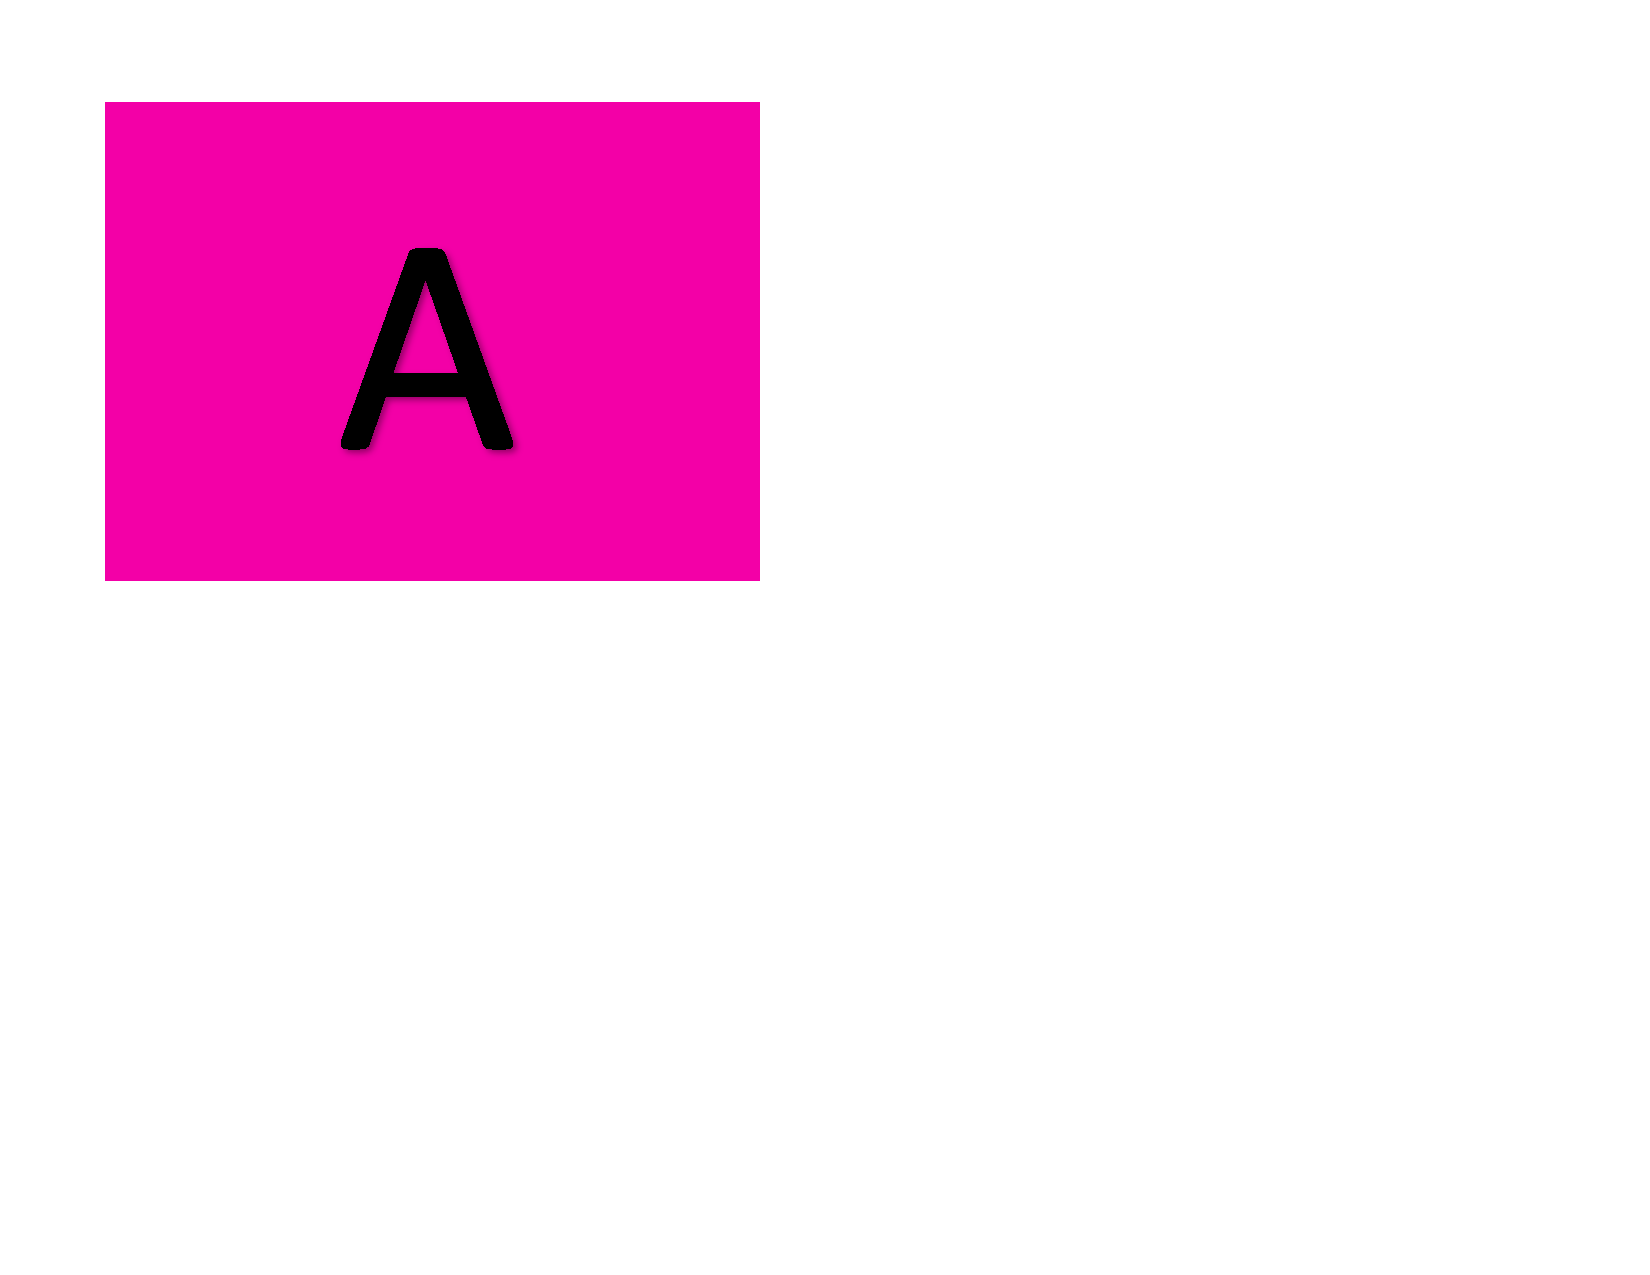
\includegraphics[width=0.8cm,height=0.5cm]{../../Lectures/figures/A}} ]  }
\newcommand*{\bitem}{ \item[{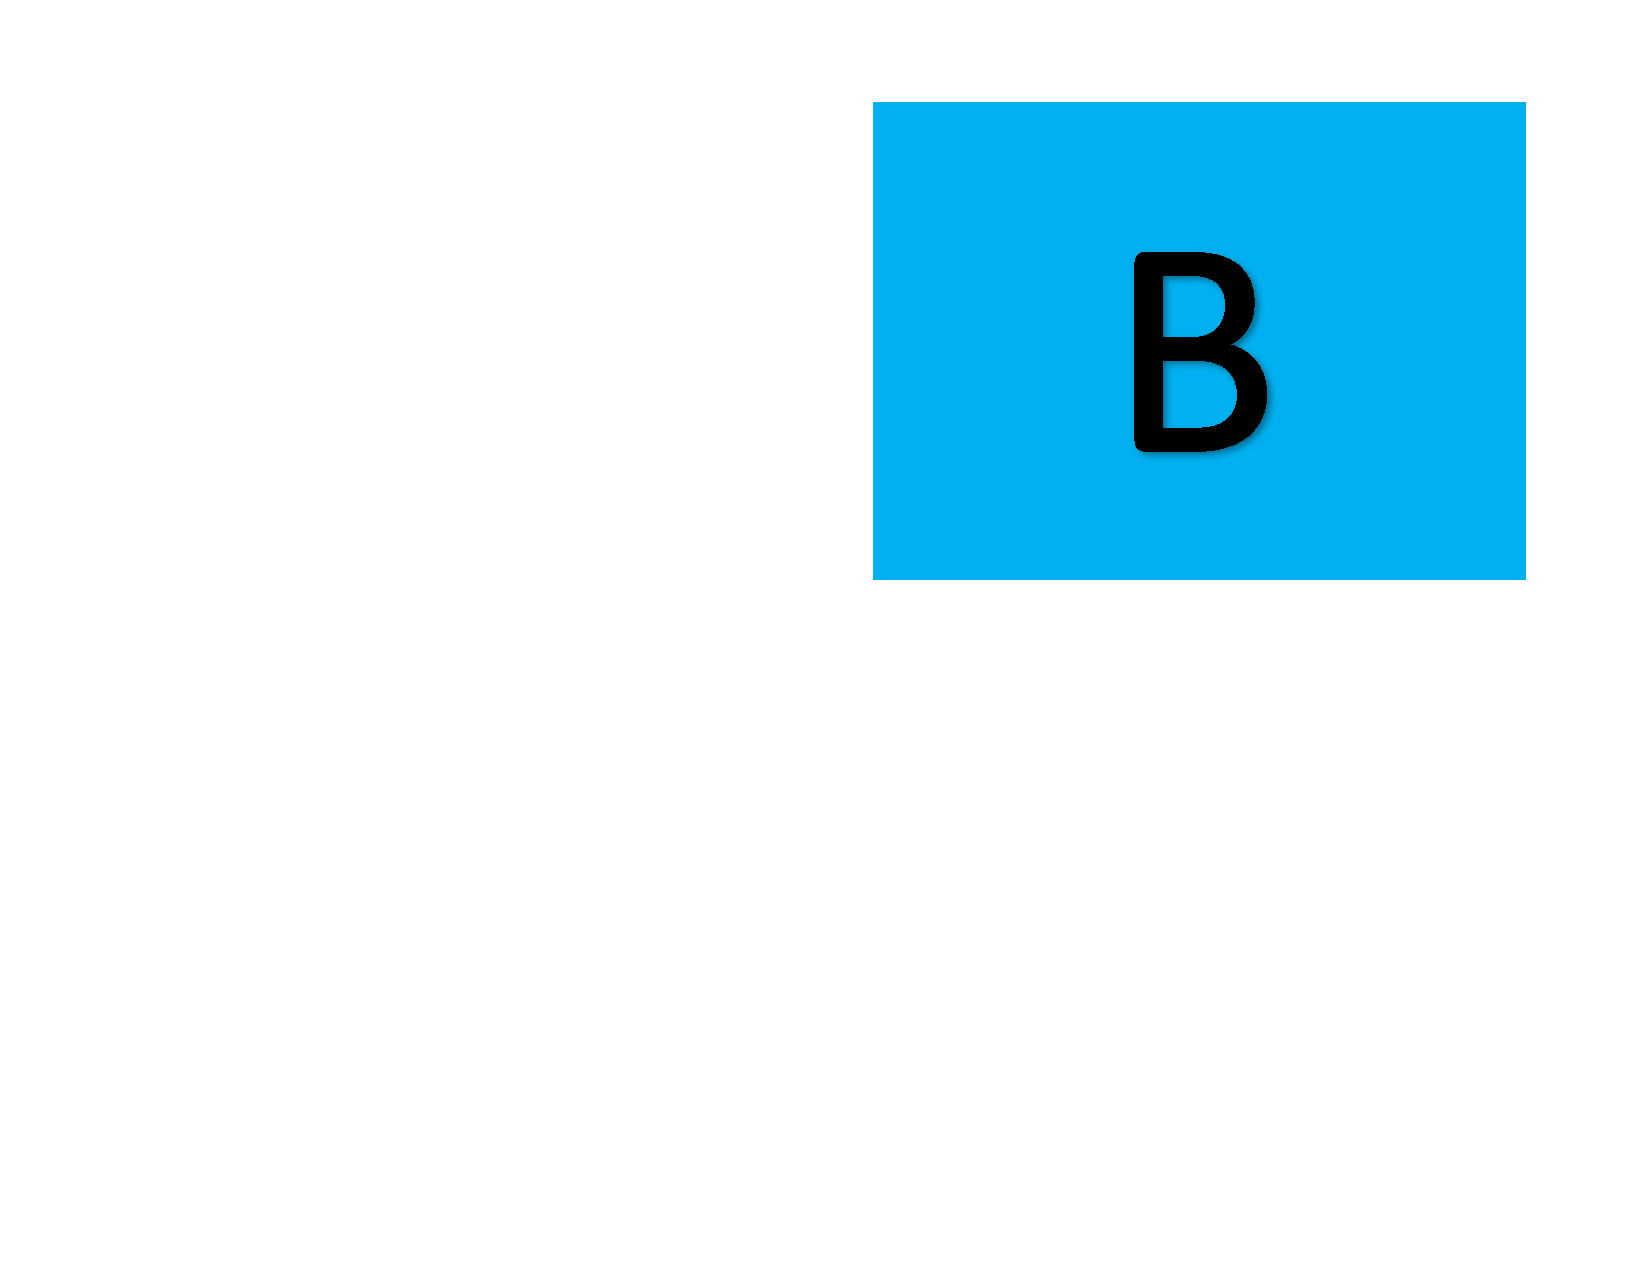
\includegraphics[width=0.8cm,height=0.5cm]{../../Lectures/figures/B}} ]  }
\newcommand*{\citem}{ \item[{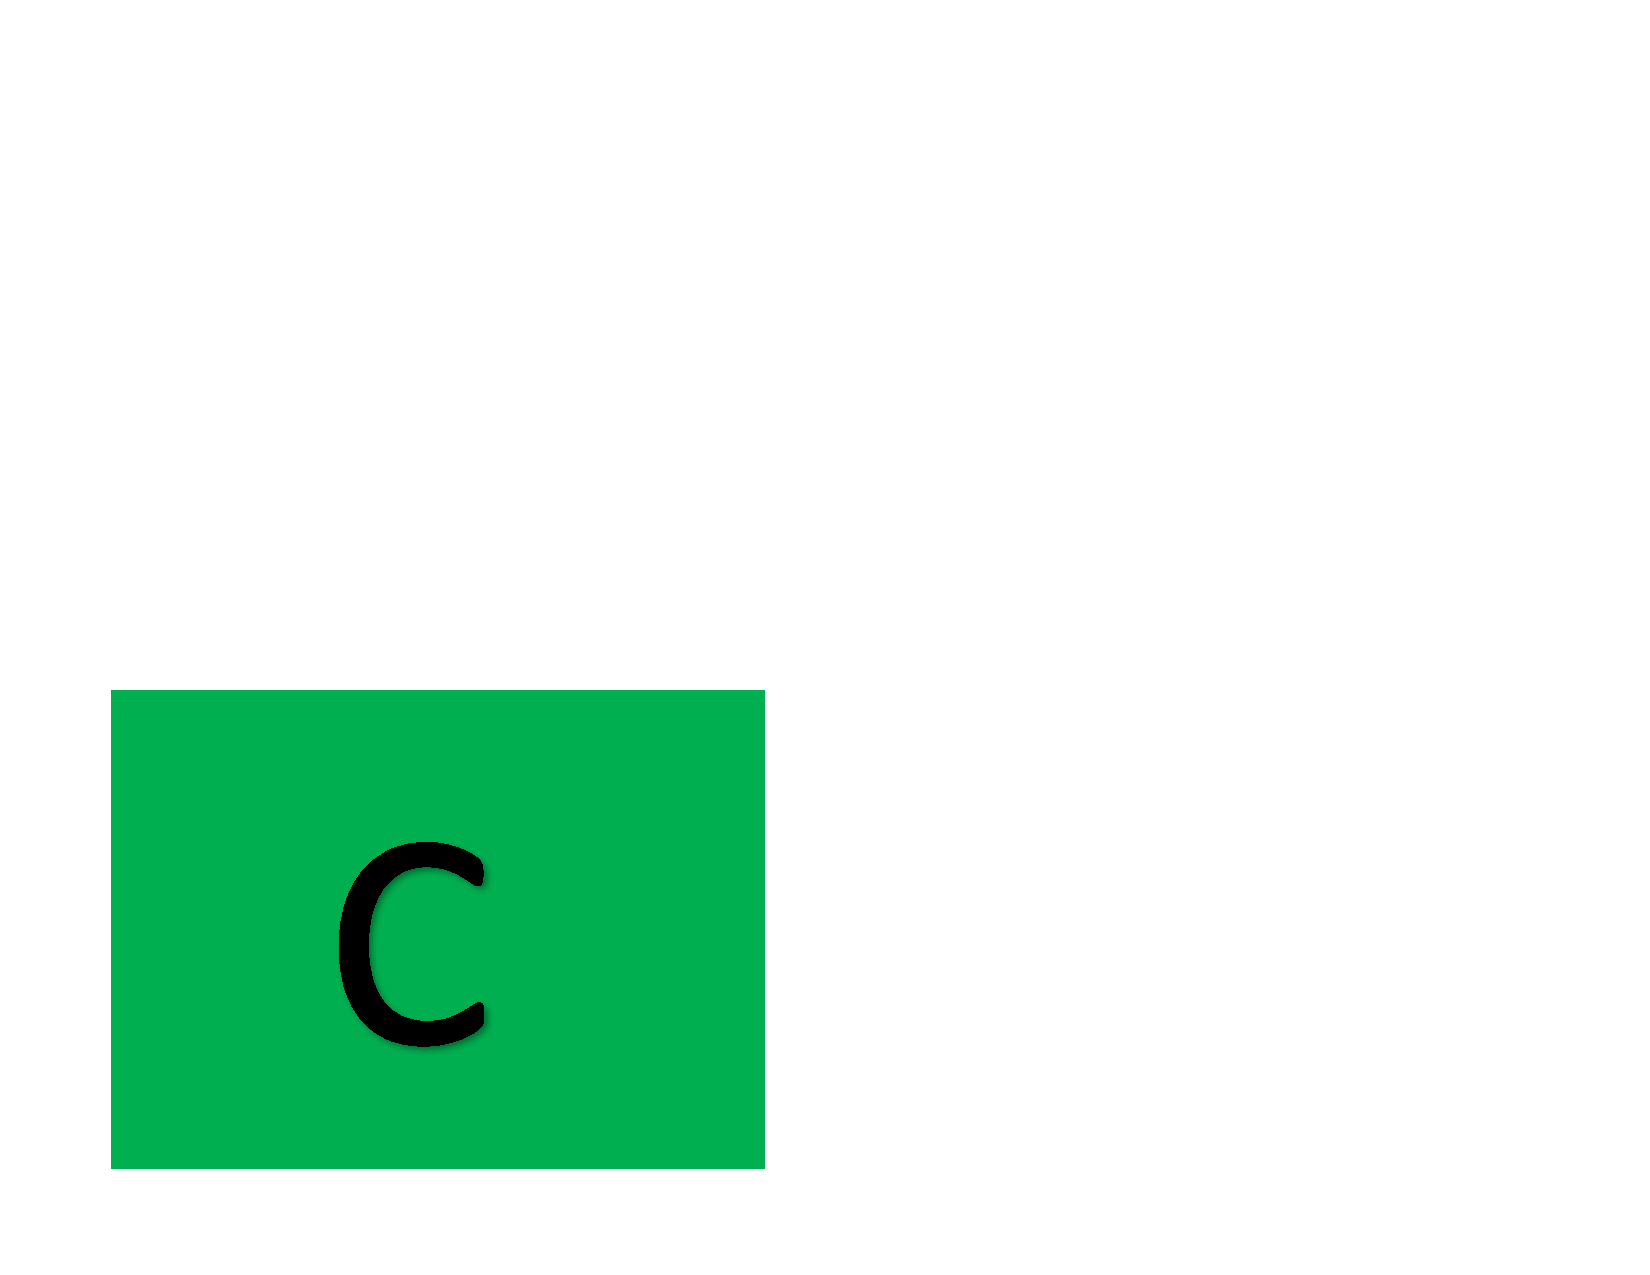
\includegraphics[width=0.8cm,height=0.5cm]{../../Lectures/figures/C}} ]  }
\newcommand*{\ditem}{ \item[{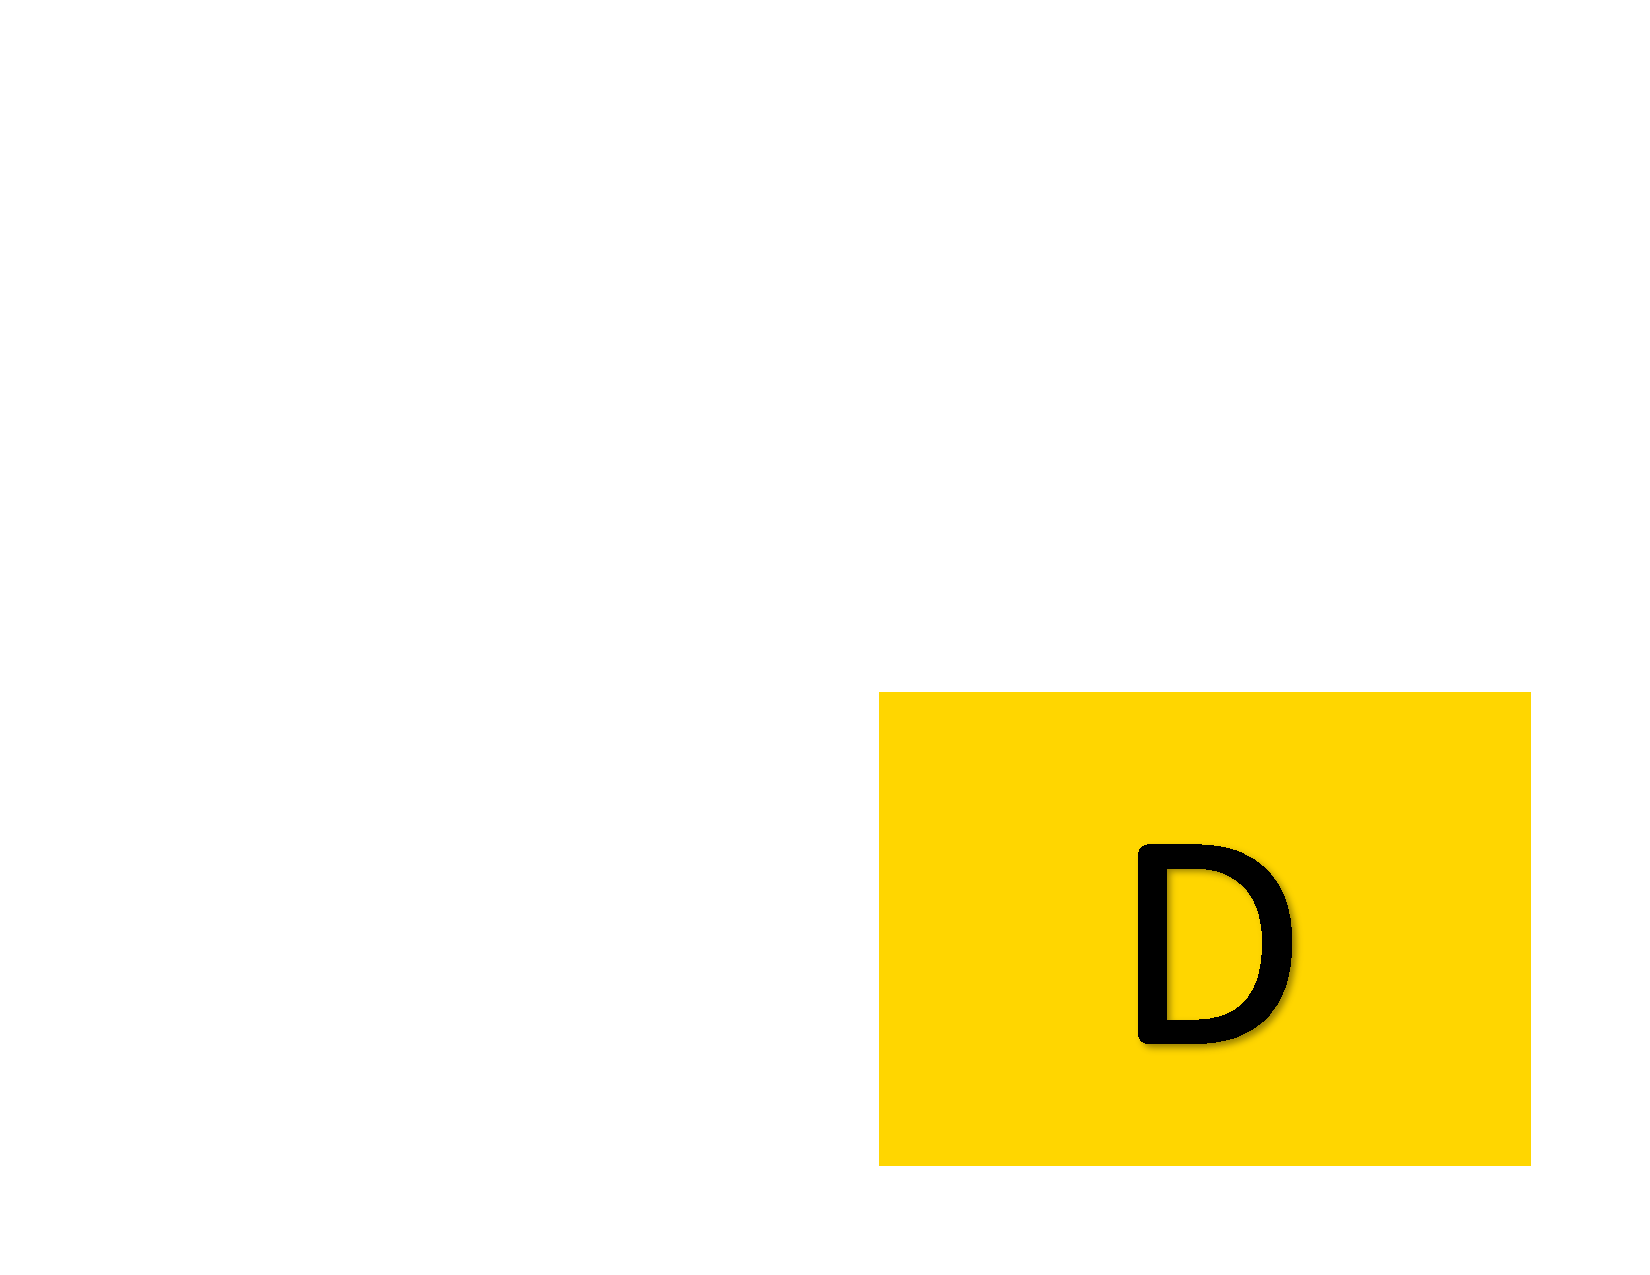
\includegraphics[width=0.8cm,height=0.5cm]{../../Lectures/figures/D}} ]  }
\newcommand*{\eitem}{ \item[{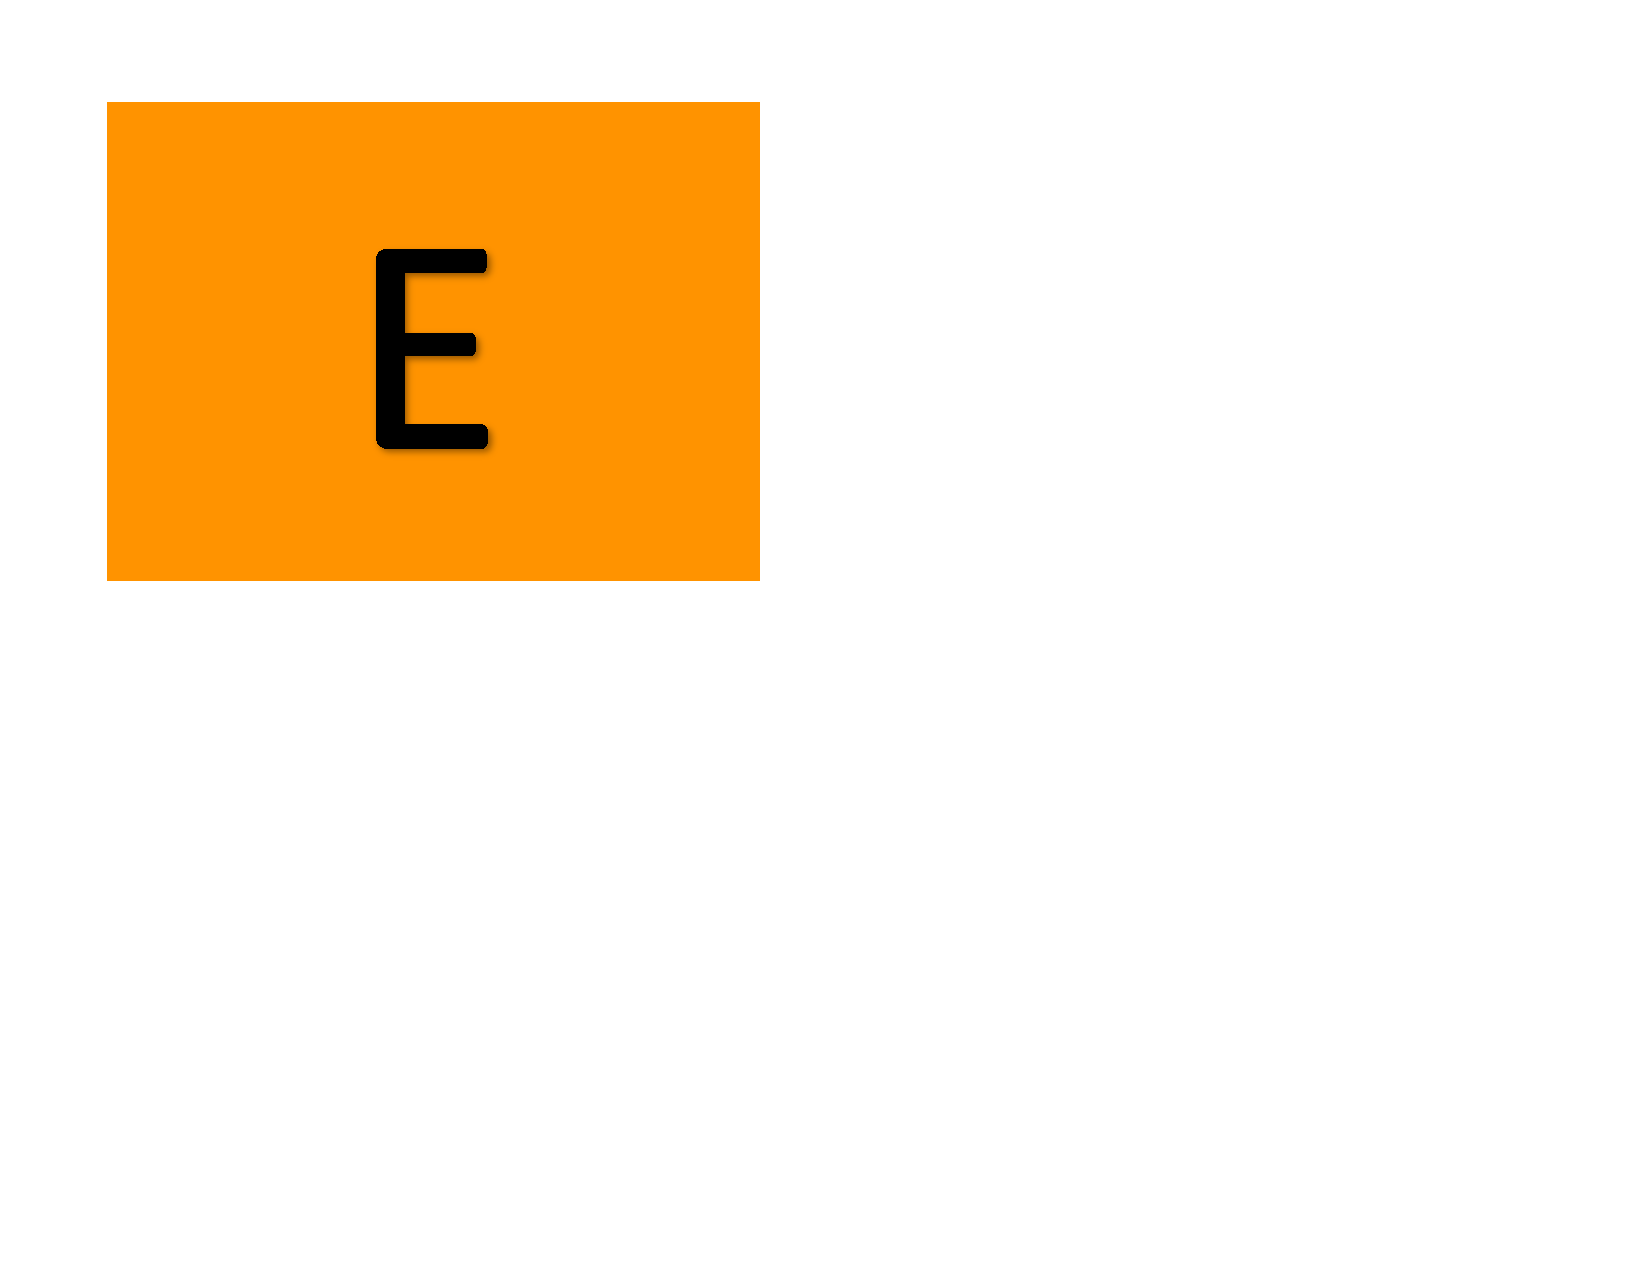
\includegraphics[width=0.8cm,height=0.5cm]{../../Lectures/figures/E}} ]  }
\newcommand*{\fitem}{ \item[{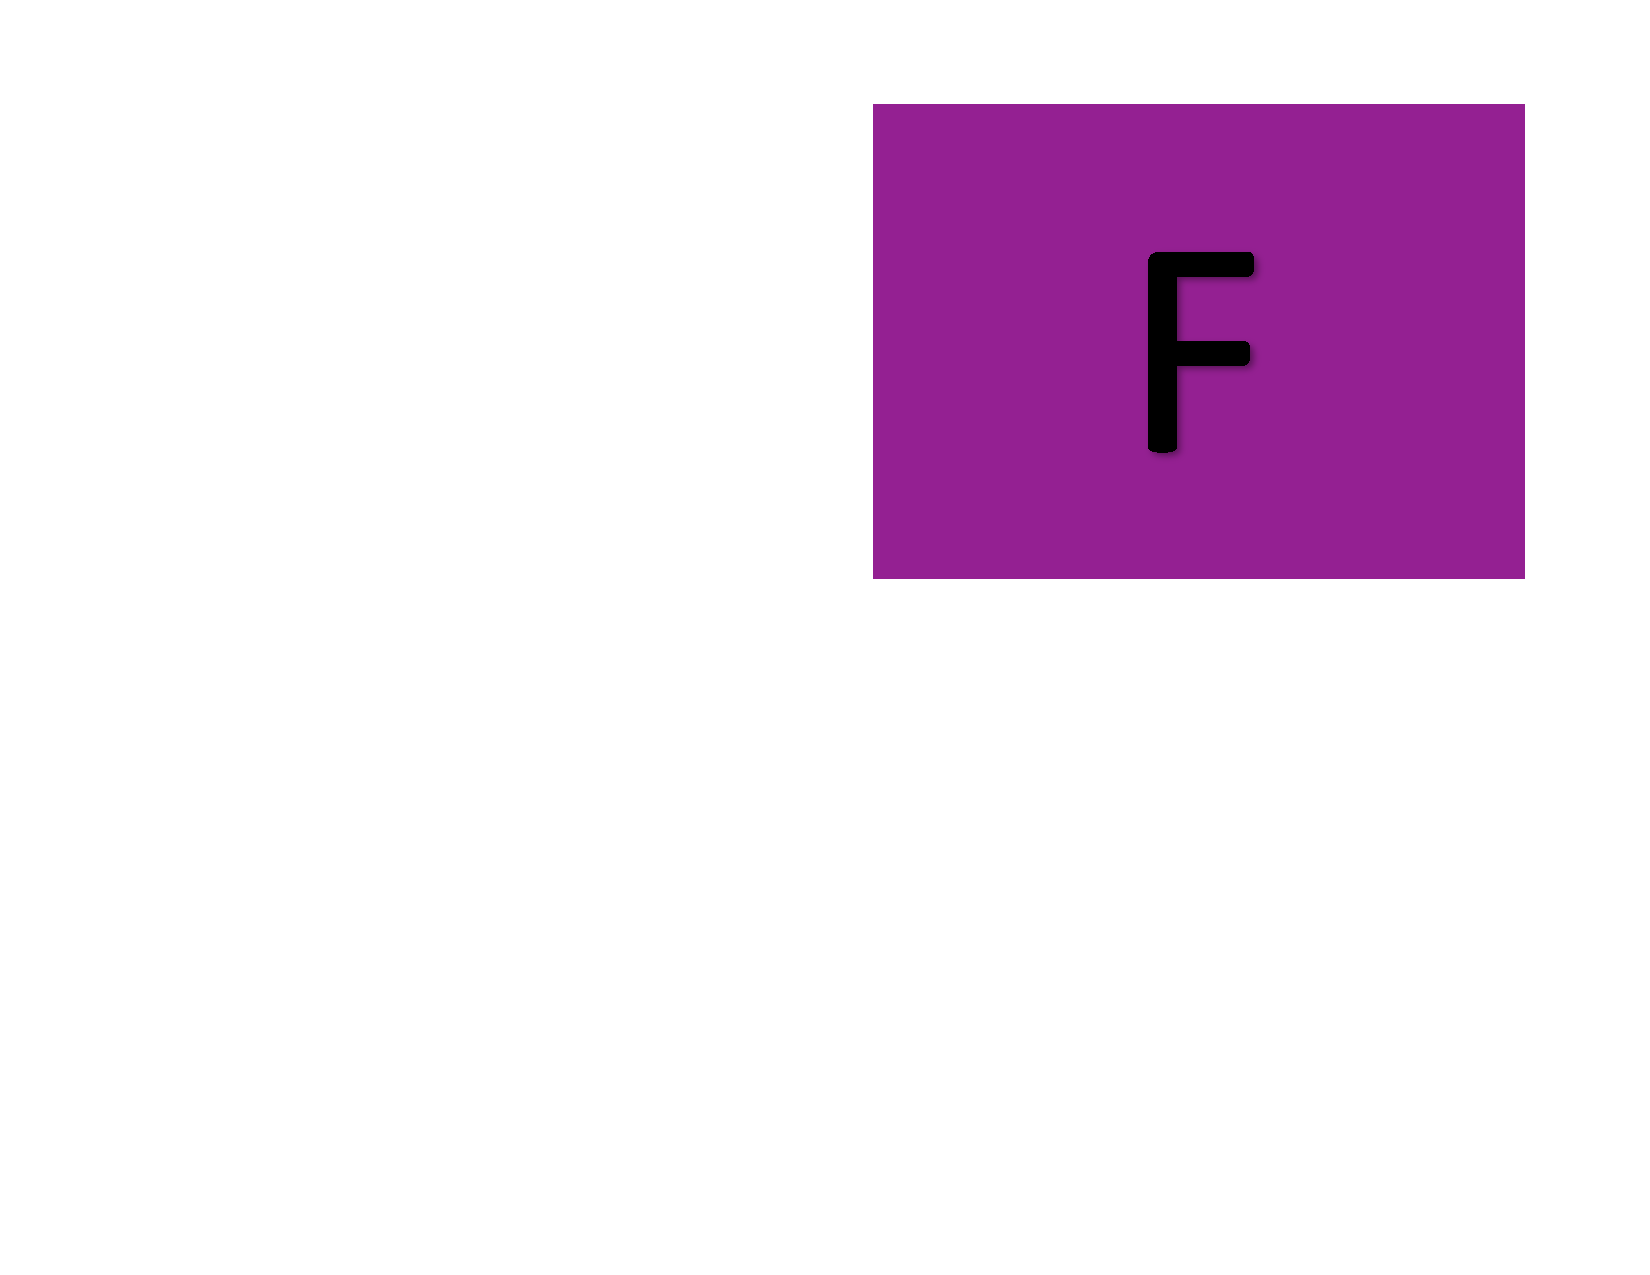
\includegraphics[width=0.8cm,height=0.5cm]{../../Lectures/figures/F}} ]  }


\newcommand{\hide}[1]{\underline{\phantom{#1 #1}}}

\usepackage{setspace}

\onehalfspacing

\begin{document}


\lecture{2: Divide and Conquer, Part II}{January 16, 2025}

	\paragraph{Course Logistics}

\begin{itemize}
	\item Read section 4.6 if you are interested in the proof of the Master Theorem.
	\item Continue skimming chapters 1-3
	\item Begin reading Chapter 15 for our next unit on Dynamic Programming
\item Syllabus quiz is due Sat, Jan 18. HW 1 and intro video due Fri, Jan 24
\end{itemize}

\section{Continued Analysis of Merge Sort}
\textbf{Merge Sort.} Given $n$ numbers to sort
\begin{itemize}
	\item Divide the sequence of length $n$ into arrays of length $\ceil{n/2}$ and $\floor{n/2}$
	\item Recursively sort the two halves
	\item (Merge Procedure) Combine the two halves by sorting them.
\end{itemize}
\QU
What is the runtime of the \emph{merge procedure} in Merge Sort?
\begin{itemize}
	\aitem $\Theta(1)$
	\bitem $\Theta(n \lg n)$
	\citem $\Theta(n)$
	\ditem $\Theta(n^2)$
\end{itemize}

\end{Qu}
\newpage

\section{Recurrence Analysis for Divide and Conquer}
Runtimes for divide and conquer algorithms can be described in terms of a \hide{recurrence} \\

relation, which \hide{lists the runtime for problem size $n$ i}\\

Let $T(n)$ denote the runtime for a problem of size $n$. \\

\paragraph{Example: merge-sort}
Assume for this analysis that $n = 2^p$ where $p \in \mathbb{N}$. \\
%\begin{equation}
%	T(n) = \begin{cases}
%		\Theta(1) & \text{if $n = 1$} \\
%		2T(n/2) + \Theta(n) & \text{if $n > 1$} \\
%	\end{cases}
%\end{equation}
%\textit{How do we turn this into a runtime?}


\newpage


\section{Three methods for solving recurrences}
Given a recurrence relation, there are three approaches to finding the overall runtime.
\begin{itemize}
\item \textbf{Recursion tree}: 
\item \textbf{Substitution method}: 
\item \textbf{Master theorem}: 
\end{itemize}

\newpage
\section{The Master Theorem for Recurrence Relations}
\begin{theorem}
	Let $a \geq 1$ and $b > 1$ be constants, let $f(n)$ be a function, and let $T(n)$ be defined on the nonnegative integers by the relation:
	\begin{equation*}
		\hide{T(n) = aT(n/b) + f(n).}
	\end{equation*}
	\begin{enumerate}
		\itemsep = 4em
		\item If $f(n) = O(n^{\log_b a - \epsilon})$ for some constant $\epsilon > 0$, then \hide{$T(n) = \Theta (n^{\log_b a })$.}
		\item If $f(n) = \Theta(n^{\log_b a})$, then \hide{$T(n) = \Theta (n^{\log_b a } \log n)$.}
		\item If $f(n) = \Omega(n^{\log_b a + \epsilon})$ for some constant $\epsilon > 0$, and if $a f(n/b) \leq c f(n)$ for some constant $c < 1$ and all sufficiently large $n$, then \hide{$T(n) = \Theta (f(n))$.}
	\end{enumerate}
\end{theorem}


\subsection{Example: Merge-Sort}

Recall that Merge-Sort satisfies the following recurrence:
\begin{equation}
	T(n) = \begin{cases}
		\Theta(1) & \text{if $n = 1$} \\
		2T(n/2) + \Theta(n) & \text{if $n > 1$} \\
	\end{cases}
\end{equation}

We can apply the master theorem with:\\

\vs{2cm} 

%$b = a$, so that $\log_b a = 1$ and $f(n) = n$.\\
%
%Then, condition 2 holds and $T(n) = \Theta (n \log n)$.

\subsection{What to know about the master method?}

\emph{Proof idea:} \\ \\%Carefully apply the recursion tree technique to the recurrence $T(n) = aT(n/b) + f(n).$\\

A full proof can be found in Section 4.6 of the textbook. \\


What's more important:  %understand what the theorem means and how to apply the master theorem.

\subsection{Examples}
Apply the master theorem to the following recurrences:
\begin{equation}
	T(n) = 9 T(n/3) + n
\end{equation}
\begin{equation}
	T(n) = 3 T(n/4) + n \log n
\end{equation}
\begin{equation}
	T(n) = 7 T(n/2) + \Theta(n^2)
\end{equation}
\newpage

\section{Strassen's Algorithm for Matrix Multiplication}

Let $A$ and $B$ be $n \times n$ matrices, and $C = AB$. The $(i,j)$ entry of $C$ is defined by
\begin{equation*}
	c_{ij} = \sum_{k = 1}^n a_{ik} b_{kj}
\end{equation*}


%In pseudocode, matrix multiplication can be written as
\begin{algorithm}[b]
	\caption{Simple Square Matrix Multiply}
	\begin{algorithmic}
		\State \textbf{Input:} $A, B \in \mathbb{R}^{n\times n}$
		\State \textbf{Output:} $C = AB \in \mathbb{R}^{n\times n}$
		\State Let $C = zeros(n,n)$
		\For{$i = 1$ to $n$}
		\For{$j = 1$ to $n$}
		\State $c_{ij} = 0$
		\For{$i = 1$ to $n$}
		\State $c_{ij} = c_{ij} + a_{ik}b_{kj}$
		\EndFor
		\EndFor
		\EndFor
		\State Return $C$
	\end{algorithmic}
\end{algorithm}

%This algorithm has a runtime of $O(n^3)$. Is it ever possible to do better?

\newpage

\subsection{An attempt at divide-and conquer}

Assume that $n = 2^p$ for some positive integer $p > 1$.


\begin{algorithm}
	\caption{Simple Recursive Square Matrix Multiply (SSMM)}
	\begin{algorithmic}
		\State \textbf{Input:} $A, B \in \mathbb{R}^{n\times n}$
		\State \textbf{Output:} $C = AB \in \mathbb{R}^{n\times n}$
		\If{$n == 1$}
		\State $c_{11} = a_{11}b_{11}$
		\Else
		\State $C_{11} = \mathit{SSMM}(A_{11},B_{11}) +   \mathit{SSMM}(A_{12},B_{21})$
		\State $C_{12} = \mathit{SSMM}(A_{11},B_{12}) +   \mathit{SSMM}(A_{12},B_{22})$
		\State $C_{21} = \mathit{SSMM}(A_{21},B_{11}) +   \mathit{SSMM}(A_{22},B_{21})$
		\State $C_{22} = \mathit{SSMM}(A_{21},B_{12}) +   \mathit{SSMM}(A_{22},B_{22})$
		\EndIf
		\State Return $C$
	\end{algorithmic}
\end{algorithm}

\QU What recursion applies to the above algorithm when $n > 1$?
\begin{enumerate}
	\aitem $T(n) = 4T(n/2) + O(n^2)$
	\bitem $T(n) = 8T(n/4) + O(n^2)$
	\citem $T(n) = 8T(n/2) + O(n)$
	\ditem $T(n) = 8T(n/2) + O(n^2)$
\end{enumerate}
\end{Qu}

\newpage

\subsection{Strassen's Algorithm}
Strassen's algorithm introduces a new way to combine matrix multiplications and additions to obtain the matrix $C$.\\

\textbf{Step 1: Partition $A$ and $B$ as before.}

\vs{3cm}


\paragraph{Step 2: Compute $S$ matrices}
\begin{align*}
&S_1 = B_{12} - B_{22} & S_2 = A_{11} + A_{12} \\
&S_3 = A_{21} + A_{22} & S_4 = B_{21} - B_{11} \\
&S_5 = A_{11} + A_{22} & S_6 = B_{11} + B_{22} \\
&S_7 = A_{12} - A_{22} & S_8 = B_{21} + B_{22} \\
&S_9 = A_{11} - A_{21} & S_{10} = B_{11} + B_{12} \\
\end{align*}

Runtime: we add (or subtract) 2 matrices of size $n/2 \times n/2$, 10 times.


\paragraph{Step 3: Compute $P$ matrices}
\begin{align*}
P_1 &= A_{11} \cdot S_1 = A_{11}\cdot B_{12} - A_{11} \cdot B_{22} \\
P_2 &= S_2 B_{22} \\
P_3 &= S_3 B_{11} \\
P_4 &= A_{22} S_4 \\
P_5 &= S_5 S_6 \\
P_6 &= S_7 S_8 \\
P_7 &= S_9 S_{10}
\end{align*}

Runtime: we recursively call the matrix-matrix multiplication function for 7 matrices of size $n/2 \times n/2$.
\newpage

\paragraph{Step 4: Combine}

Using the $P$ matrices, we can show that\\

$
C_{11} = P_5 + P_4 - P_2 + P_6 \\
C_{12} = P_1 + P_2 \\
C_{21} = P_3 + P_4 \\
C_{22} = P_5 + P_1 - P_3 - P_7
$

\newpage
\subsection{Analysis of Strassen's Method}
\QU Strassen's algorithm satisfies which recurrence relation for $n > 1$?
\begin{enumerate}
\aitem $T(n) = 8T(n/2) + O(n^2)$
\bitem $T(n) = 23T(n/2)$
\citem $T(n) = 7T(n/2) + O(n^2)$
\ditem $T(n) = 10T(n/2) + O(n^2)$
\eitem $T(n) = 17T(n/2) + O(1)$
\end{enumerate}
\end{Qu}



\end{document}
